%%%%%%%%%%%%%%%%%%%%%%%%%%%%% Define Article %%%%%%%%%%%%%%%%%%%%%%%%%%%%%%%%%%
\documentclass[12pt]{article}
%%%%%%%%%%%%%%%%%%%%%%%%%%%%%%%%%%%%%%%%%%%%%%%%%%%%%%%%%%%%%%%%%%%%%%%%%%%%%%%

%%%%%%%%%%%%%%%%%%%%%%%%%%%%% Using Packages %%%%%%%%%%%%%%%%%%%%%%%%%%%%%%%%%%
\usepackage{geometry}
\usepackage{graphicx}
\usepackage{amssymb}
\usepackage{amsmath}
\usepackage{amsthm}
\usepackage{empheq}
\usepackage{mdframed}
\usepackage{booktabs}
\usepackage{lipsum}
\usepackage{color}
\usepackage{psfrag}
\usepackage{pgfplots}
\usepackage{bm}
\usepackage[export]{adjustbox}
\usepackage{float}
\usepackage{enumitem}
\usepackage{pythonhighlight}
%%%%%%%%%%%%%%%%%%%%%%%%%%%%%%%%%%%%%%%%%%%%%%%%%%%%%%%%%%%%%%%%%%%%%%%%%%%%%%%

% Other Settings

%%%%%%%%%%%%%%%%%%%%%%%%%% Page Setting %%%%%%%%%%%%%%%%%%%%%%%%%%%%%%%%%%%%%%%
\geometry{
  a4paper,
  total={170mm,257mm},
  left=0.75in,
  right=0.75in,
  top=0.75in,
  bottom=0.75in,
}

\setlist[itemize]{itemsep=-2pt}
\setlist[enumerate]{itemsep=-2pt}
\setlength{\parindent}{0px}

%%%%%%%%%%%%%%%%%%%%%%%%%% Define some useful colors %%%%%%%%%%%%%%%%%%%%%%%%%%
\definecolor{ocre}{RGB}{243,102,25}
\definecolor{mygray}{RGB}{243,243,244}
\definecolor{deepGreen}{RGB}{26,111,0}
\definecolor{shallowGreen}{RGB}{235,255,255}
\definecolor{deepBlue}{RGB}{61,124,222}
\definecolor{shallowBlue}{RGB}{235,249,255}
%%%%%%%%%%%%%%%%%%%%%%%%%%%%%%%%%%%%%%%%%%%%%%%%%%%%%%%%%%%%%%%%%%%%%%%%%%%%%%%

%%%%%%%%%%%%%%%%%%%%%%%%%% Define an orangebox command %%%%%%%%%%%%%%%%%%%%%%%%
\newcommand\orangebox[1]{\fcolorbox{ocre}{mygray}{\hspace{1em}#1\hspace{1em}}}
%%%%%%%%%%%%%%%%%%%%%%%%%%%%%%%%%%%%%%%%%%%%%%%%%%%%%%%%%%%%%%%%%%%%%%%%%%%%%%%

%%%%%%%%%%%%%%%%%%%%%%%%%%%% English Environments %%%%%%%%%%%%%%%%%%%%%%%%%%%%%
\newtheoremstyle{mytheoremstyle}{3pt}{3pt}{\normalfont}{0cm}{\rmfamily\bfseries}{}{1em}{{\color{black}\thmname{#1}~\thmnumber{#2}}\thmnote{\,--\,#3}}
\newtheoremstyle{myproblemstyle}{3pt}{3pt}{\normalfont}{0cm}{\rmfamily\bfseries}{}{1em}{{\color{black}\thmname{#1}~\thmnumber{#2}}\thmnote{\,--\,#3}}
\theoremstyle{mytheoremstyle}
\newmdtheoremenv[linewidth=1pt,backgroundcolor=shallowGreen,linecolor=deepGreen,leftmargin=0pt,innerleftmargin=20pt,innerrightmargin=20pt,]{theorem}{Theorem}[section]
\theoremstyle{mytheoremstyle}
\newmdtheoremenv[linewidth=1pt,backgroundcolor=shallowBlue,linecolor=deepBlue,leftmargin=0pt,innerleftmargin=20pt,innerrightmargin=20pt,]{definition}{Definition}[section]
\theoremstyle{myproblemstyle}
\newmdtheoremenv[linecolor=black,leftmargin=0pt,innerleftmargin=10pt,innerrightmargin=10pt,]{problem}{Problem}[section]
%%%%%%%%%%%%%%%%%%%%%%%%%%%%%%%%%%%%%%%%%%%%%%%%%%%%%%%%%%%%%%%%%%%%%%%%%%%%%%%

%%%%%%%%%%%%%%%%%%%%%%%%%%%%%%% Plotting Settings %%%%%%%%%%%%%%%%%%%%%%%%%%%%%
\usepgfplotslibrary{colorbrewer}
\pgfplotsset{width=8cm,compat=1.9}
%%%%%%%%%%%%%%%%%%%%%%%%%%%%%%%%%%%%%%%%%%%%%%%%%%%%%%%%%%%%%%%%%%%%%%%%%%%%%%%

%%%%%%%%%%%%%%%%%%%%%%%%%%%%%%% Title & Author %%%%%%%%%%%%%%%%%%%%%%%%%%%%%%%%
\title{Computer Vision}
\author{Laxman Desai}
%%%%%%%%%%%%%%%%%%%%%%%%%%%%%%%%%%%%%%%%%%%%%%%%%%%%%%%%%%%%%%%%%%%%%%%%%%%%%%%

\begin{document}

\maketitle
\tableofcontents

\pagebreak
\section{Optical Character Recognition}

  We will try and build a model that can break CAPTCHAs. What's a CAPTCHA? It's basically a the test to determine if the user is a bot or a human. We will first attempt at breaking text based CAPTCHAs.
  
  \paragraph{Stages:}
  \begin{enumerate}
    \item Data acquisition
    \item Preprocessing
    \item Building a model
    \item Training the model
    \item Testing the model
  \end{enumerate}

  \subsection{Preprocessing}
    We cannot input an image directly for the OCR system. Some pre-processing has to be done on the image so that it becomes easy for the OCR model to recognize the information in the image.

    \paragraph{Preprocessing includes the following:}
    \begin{enumerate}
      \item Skew Correction
      \item Removing Lines (Horizontal \&  Vertical)
      \item Building a model
      \item Testing
    \end{enumerate}
    
    \subsubsection{Skew Correction}
      Image obtained from the previous stage may not be correctly oriented, It may be aligned at any angle. So we need to perform skew correction to make sure that the image forwarded to subsequent stages is correctly oriented.
      
      \begin{figure}[H]
        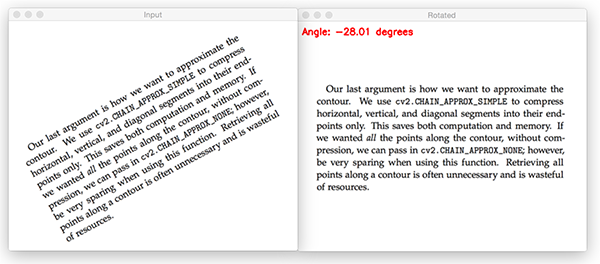
\includegraphics[width=0.75\textwidth, center]{images/2.png}
        \caption{Picture caption}
      \end{figure}
    
    \subsubsection{Binarization}
      That is, converting a coloured image to a black and white binary image. In practice, there exists an intermediate grayscale image.
      
      \begin{equation*}
        \text{Coloured image} \rightarrow \text{Grayscale image} \rightarrow \text{Binary image}
      \end{equation*}
      
      \begin{figure}[H]
        \centering
        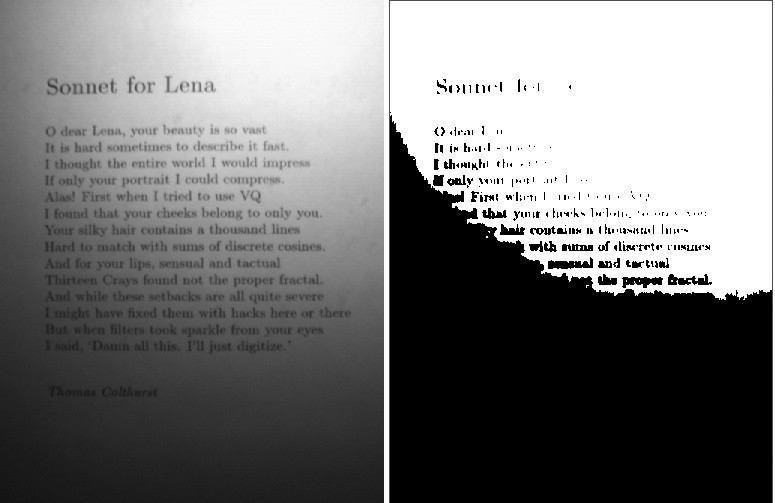
\includegraphics[width=0.75\textwidth]{images/1.jpeg}
        \caption{Binarization using a threshold on the image captured under non-uniform lighting.}
      \end{figure}

      Converting an RGB image to a grayscale image is easy. 
      To a computer, a black pixel has a value of 0 and a white pixel has a value of 255. Converting a grayscale to B\&W requires one to set a threshold value. If the pixel value is greater than the threshold, it is considered as a white pixel, else its as a black pixel. This naive strategy fails when lighting conditions are not uniform in the image. Here we can use Otsu's method or adaptive thresholding.
      
      \paragraph{Otsu's Binarization:}
      Since we are working with bimodal images, Otsu's algorithm tries to find a threshold value (t) which minimizes the weighted within-class variance given by the relation:
      
      \begin{equation*}
        \sigma_w^2(t) = q_1(t)\sigma_1^2(t)+q_2(t)\sigma_2^2(t)
      \end{equation*}
      
      where,
      
      \begin{align*}
        q_1(t) = \sum_{i=1}^{t} P(i) \quad &\& \quad q_2(t) = \sum_{i=t+1}^{I} P(i)
        \\
        \mu_1(t) = \sum_{i=1}^{t} \frac{iP(i)}{q_1(t)} \quad &\& \quad \mu_2(t) = \sum_{i=t+1}^{I} \frac{iP(i)}{q_2(t)}
        \\
        \sigma_1^2(t) = \sum_{i=1}^{t} [i-\mu_1(t)]^2 \frac{P(i)}{q_1(t)} \quad &\& \quad \sigma_2^2(t) = \sum_{i=t+1}^{I} [i-\mu_2(t)]^2 \frac{P(i)}{q_2(t)}
      \end{align*}
      
      \paragraph{Python code:} \
      \begin{python}
        import cv2 as cv

        # global thresholding
        ret1,th1 = cv.threshold(img,127,255,cv.THRESH_BINARY)

        # Otsu's thresholding
        ret2,th2 = cv.threshold(img,0,255,cv.THRESH_BINARY+cv.THRESH_OTSU)

        # Otsu's thresholding after Gaussian filtering
        blur = cv.GaussianBlur(img,(5,5),0)
        ret3,th3 = cv.threshold(blur,0,255,cv.THRESH_BINARY+cv.THRESH_OTSU)
      \end{python}
        
    \subsubsection{Removing Lines (Horizontal \& Vertical)}
      

\end{document}